\documentclass[12pt, a4paper]{article}

\usepackage{tgbonum}
\usepackage{blindtext}

\usepackage{xcolor}
\usepackage{graphicx}
\usepackage{multicol}

\usepackage[mode=buildnew]{standalone}% requires -shell-escape
\usepackage{tikz}

\begin{document}
	
% TITLE PAGE
\thispagestyle{empty}
{ \centering
	CERN
	\vspace*{0.5cm}
	
	\footnotesize
	Summer Student Project Report\\
	\huge
	{\sc Converting Solids to VecGeom's Surface Model}\\
	\vspace{0.4cm}
	\footnotesize
	\begin{tabular}{l c r}
		student: & \hspace{3cm}\ & supervisor:\\
		Dušan Cvijetić\footnotemark, && Dr. Andrei Gheata, \\
		\scriptsize University of Belgrade && \scriptsize CERN EP-SFT
	\end{tabular}
	\footnotetext{\fontfamily{qcr}\selectfont dusancvijetic2000@gmail.com}
	
	\normalsize
	\vspace{0.5cm}
	Geneve,\\
	\today
		
	
}

\vfill
\begin{abstract}
	\blindtext
\end{abstract}
\vfill

\newpage


\tableofcontents

\section{Introduction}

Simulating geometry is a necessary part of any detector simulation in high energy physics. It introduces constraints to a given problem, bounding physical properties to regions of space.

One of the most important tasks geometry model has is navigation of moving particles. It must provide information on where the particle currently is, so that interactions with material can be properly simulated, but also predict where will the particle hit boundary of the current region. This prediction is done through checking ray--boundary intersections, so as to see whether the particle's trajectory leads it to exit the current region and pass into another.

Traditionally, this was done for a single particle and a single potential intersection. However, with the advent of powerful GPU technologies in the recent years, a question arises if there is possibility for parallelization, and therefore speedup, of this process. As the simulation of particle movement is one of the most resource-intensive tasks of collision simulations, its acceleration would be very valuable. VecGeom library is an effort in this direction.

Old models used the concept of solids (3D volumes) to represent the elements of a detector. However, GPU parallelization over the solid structures turns out to be quite inefficient, for they tend to use many registers and exhibit a lot of divergence. A promising approach to solving these problems is decomposing the volumes into surfaces, lowering register usage and producing less divergent algorithms.


\section{Bounded Surface Model}

There are a few approaches to implementing surface models for geometry simulations, including triangulation or half-space decomposition. VecGeom, however, uses the bounded surface model.

To create a shape in this model, it is necessary to decompose a solid into its limiting surfaces. At first, infinite surfaces are generated. Creating a useful structure from infinite surfaces is then done by using frames, which delimit the area that really exist from the virtual one (figure \ref{fig:mask}). If a particle is traveling through space and hits the surface, it also has to check if it has landed within the frame. If not, then the collision wasn't real and should be ignored. If yes, then the surface was really hit and it should be checked how this affects the particle's state (i.e. what are the two regions between which a particle is crossing through a surface).
\begin{figure}[h]
	\centering
	\includestandalone[width = 0.4\textwidth]{Figures/cylinder3_construction}
	\caption{Frame on an infinite cylinder creates a framed cylindrical surface.}
	\label{fig:mask}
\end{figure}

Depending on the setup, it may happen that certain surfaces lie in each other's extensions. Planes might share a common normal (figure \ref{fig:commonSurf}), or cylinders might have the same axes and radii. In such cases, it is useful to group these smaller structures into a common surface object.
\begin{figure}[h]
	\centering
	\includestandalone[width = 0.7\textwidth]{Figures/extents}
	\caption{Masked planar surfaces that share a common normal.}
	\label{fig:commonSurf}
\end{figure}

A common surface is, just like before, created so that it extends to infinity. That is not very practical, and a way must be found to delimit the useful area from its virtual part. Unlike before, when frames were used to limit the surfaces based on solid's parameters, the useful part of a common surface is determined by the placement and masks of framed surfaces that make it.

To delimit common surfaces, a structure called extent is used. Extents are akin to frames, only they represent "bounding boxes" for all framed surfaces on a common surface. They are the predefined geometrical structures with smallest possible area that covers all the frames. (Figure \ref{fig:extent})
\begin{figure}[h]
	\centering
	\includestandalone[width = 0.7\textwidth]{Figures/extents2}
	\caption{Rectangular extent on a planar common surface. At first, all that the particle sees is an extent. Frames are checked only if the extent is hit.}
	\label{fig:extent}
\end{figure}

The purpose of an extent is to cut down the number of frames that have to be checked. When a particle is traversing the space and can potentially hit a certain common surface, the first step is to check whether its trajectory intersects the common surface within its extent. If not, then there is no possibility that the particle will hit any of the framed surfaces, and their frames don't have to be checked separately. Since it is much more common for a particle not to hit within an extent than to hit it, this optimization provides substantial speedup to the navigating algorithm.

Two framed surfaces can also lie on a same common surface and have opposite orientations (i.e. two planes with parallel normals that point in opposite directions). Such cases are treated by decomposing a common surface into two sides. The extents, then, are computed for each side, and not for the whole common surface, and which side should be checked is determined by navigation algorithm.


\section{Implementation}

The implementation of described structure in a way that can run on both CPU and GPU presents many constraints. For one, all structures and functions must be templated, so that appropriate data types can be used depending on architecture the code is running on. Dynamic memory allocation cannot be used in algorithms meant to run on GPU. Inheritance mechanism also cannot be utilized, and so virtual functions can't be created.


\subsection{The old architecture}

The initial architecture of Surface Model library was in its prototypal phase. There was some confusion with structure names, the delegation of responsibility was in many places inappropriate, and overall scalability was quite bad. The restructuring had to be done for further development to be possible.

All the data needed for geometry was stored within SurfData structure. This allows greater control over memory allocation and better GPU compatibility. On top of that, various structures were implemented to represent the elements of the surface model: RangeMask, Extent, UnplacedSurface, Frame, FramedSurface, Side and CommonSurface.

//TODO: UML diagram of old architecture.

RangeMask structure had two real numbers as its members, and was meant for data storage. It implemented a few basic operations, like getting and setting its members. Transformation was a class for moving around the produced surfaces into their places.

Extent data structure was comprised of two RangeMasks and was meant to represent various types of both frames and extents. This introduced confusion about its purpose, and produced messy and repetitive code (for example, the same checks had to be made for both Frame and CommonSurface structures). The limitation of using only two Range objects to represent any possible frame or extent resulted in impossibility to specialize structures based on their purpose. To some extent, it was possible to bypass this limitation through specializing generation algorithms, but even when such hacks were utilized, some shapes still couldn't fit into four real numbers however ingenious the conjured solution was. This structure was the main culprit of many problems that arose throughout development.

UnplacedSurface represented infinite surfaces before they were framed.

Frame provided more general interface for connecting the UnplacedSurfaces with Extent objects. It kept the info about the Extent type and the Extent itself as its members. The algorithm for checking if the point lies within the extent was implemented inside the Frame in two variants: one was meant for framed surfaces, and the other, static one, for checking extents on common surfaces.

FramedSurfaces were used to connect Frames with UnplacedSurfaces. Sides and CommonSurfaces were used for grouping of FramedSurfaces, as told before. Sides used Extents for delimiting the useful area.


\subsection{The new architecture}

The new architecture used for implementation of surface model had to be scalable, as new types of objects should eventually be supported by the library. This was provided through better object decomposition and delegation of responsibility.

Range structure was done away with, and replaced by more general Vec2D structure, with some new operations implemented (such as vector subtraction or quasi cross product for z-component calculation). Depending on the use case, Vec2D was aliased as Range, Point2D, or AngleVector. 

The major restructuring was done on frames and extents. Firstly, the new structures, called Masks, were introduced. Masks serve as low-level implementations of various possible shapes that frames and extents can take, allowing for specialization of different types. All mask structures, apart from constructor, have an {\fontfamily{qcr}\selectfont Inside()} member function, whose purpose is to check if a given point lies within mask's shape. Currently, there are only five masks implemented:
\begin{description}
	\item [WindowMask] represents a rectangular mask on a planar surface;
	\item [RingMask] represents a surface extending between two circular segments, one with radius $r_{min}$ and the other $r_{max}$, starting at an angle $\varphi_{min}$ and extending to $\varphi_{max}$;
	\item [ZPhiMask] represents a mask delimiting a cylindrical surface segment along z-axis, starting from $z_{min}$ and extending to $z_{max}$, and spanning between angles $\varphi_{min}$ and $\varphi_{max}$;
	\item[TriangularMask\footnotemark] represents a triangular mask on a planar surface and
	\item[QuadrilateralMask] represents a convex quadrilateral mask on a planar surfacel,
\end{description}
but the number of mask types should still grow.
\footnotetext{These have not been tested yet.}

\begin{figure}[h]
	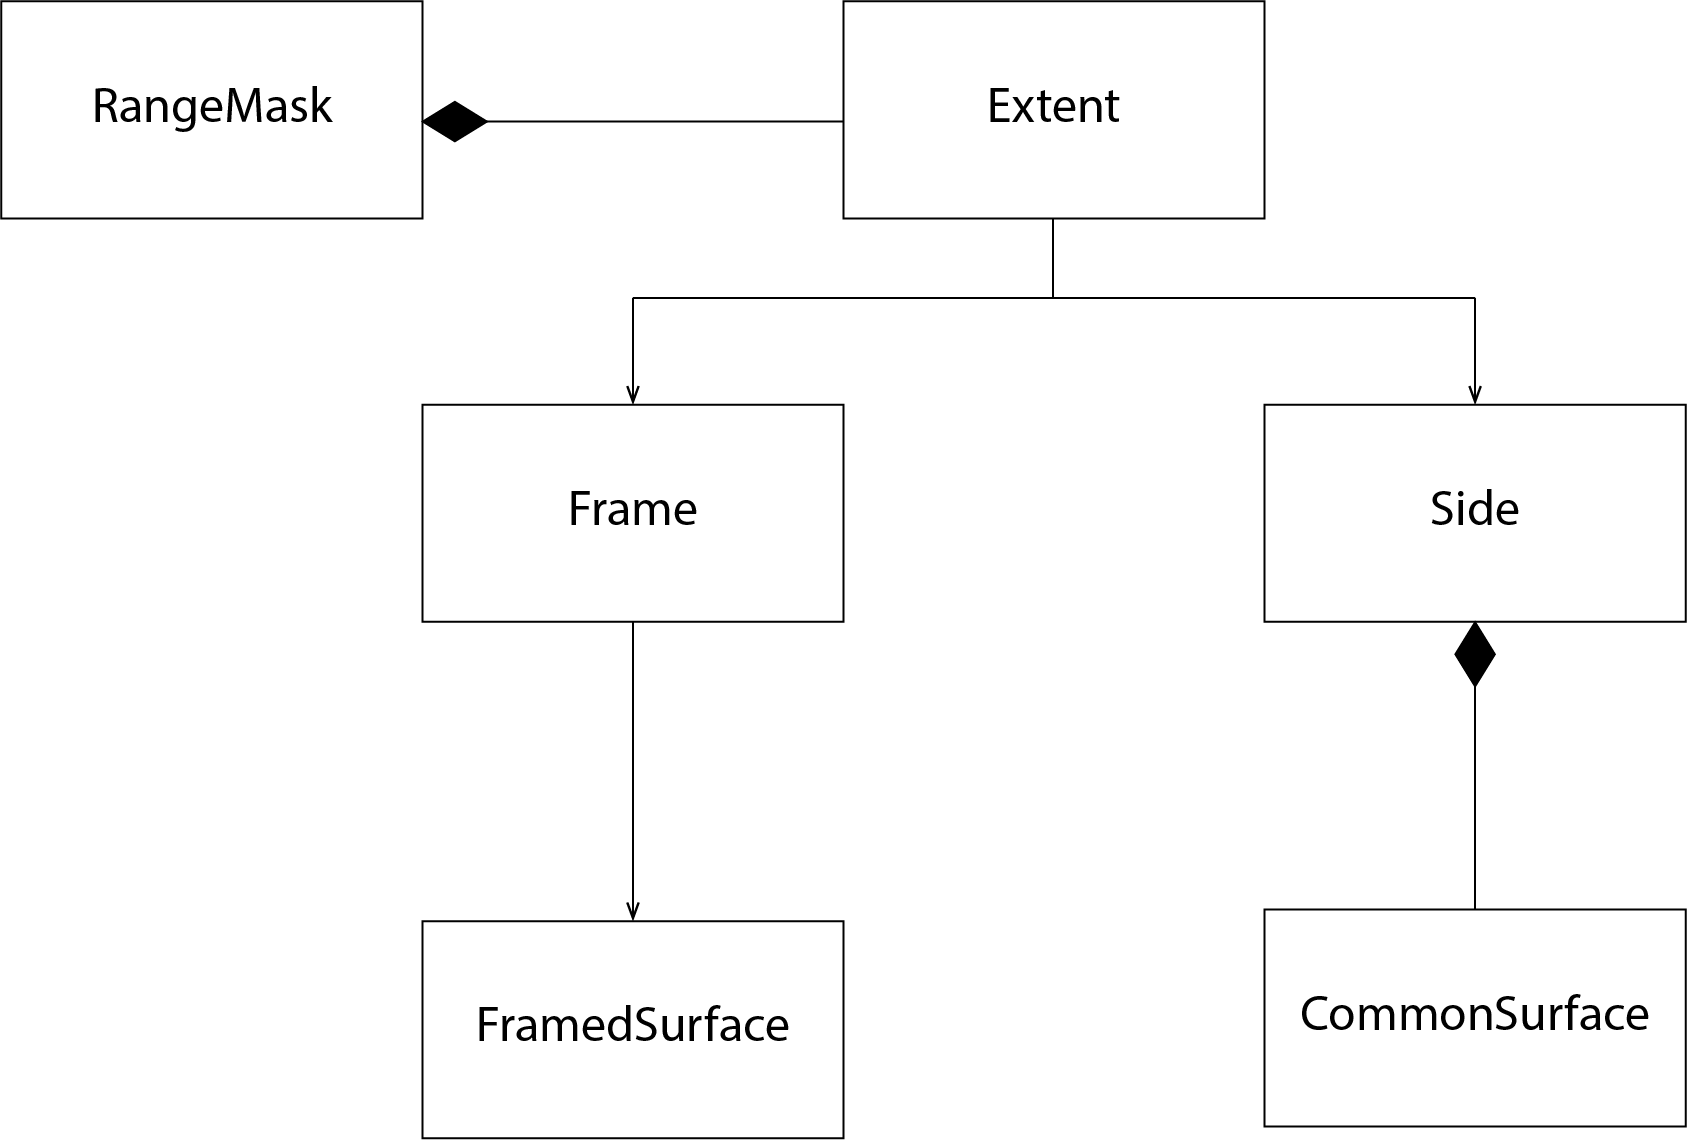
\includegraphics[width=\textwidth]{Figures/diagram_old.png}
	\caption{Architecture after redesign. Mask structure doesn't really exist, because virtual mechanism cannot be utilized. It is just an illustration of similarity between different mask structures, and not a real parent.}
\end{figure}

The Frame remains as an interface between Mask and Surface. Since the usage of virtual mechanism was not allowed, selecting the right {\fontfamily{qcr}\selectfont Inside()} function for applied mask is done through a switch statement in Frame structure's own {\fontfamily{qcr}\selectfont Inside()} function. Case is selected based on a mask type, a parameter that is stored as data member.

On Sides, extents are now not implemented as a special class, but rather as an aliased Frame objects. That way, there is much less code duplication, and logically the same mechanisms are kept as a single piece of code. This also allows Masks to be used on both UnplacedSurfaces (through Frames) and Sides. The type of a mask on an extent is enforced upon extent's creation, so that the planar sides will always be delimited by WindowMasks, and Cylinders by ZPhiMasks.

With these modifications, model's scalability was increased, and it has become more straightforward to implement new masks and solid-surface conversions.


\section{Implementing shapes}

\subsection{Tube}

The only solid-to-surface conversion that was already done at the start of this project was for cube solids. Implementing tube surfaces posed a few new challenges.

In general, tubes occupy region delimited by two coaxial cylinders with different radii, between some non-zero non-equal starting and ending angles, and with finite length along axis. If the angles are equal, the tube's cross section is a full circle. If inner radius is zero, the tube is not hollow.

Firstly, an algorithm was written for calculating the distance between a point in space and cylindrical surface along a given direction. As only the planes have been implemented earlier, this was the first second-order system of equations that needed to be solved, and the simple and fast quadratic equation solver was implemented.

RingMasks and ZPhiMasks were introduced for framing surfaces that constitute tube. In general, there were six of those: outer and inner cylindrical surfaces with ZPhiMasks, top and bottom cap with RingMasks and two planar sides for covering the phi-cut of the cylinder with WindowMasks.


\subsection{Trapezoidal prism}

Another new solid whose conversion has been implemented is trapezoidal prism. It consists of top and bottom planar surfaces with rectangular masks of (in general) different sizes, and four planar side surfaces with quadrilateral masks. The optimization was introduced so that WindowMasks are created instead of QuadrilateralMasks whenever possible, since running the {\fontfamily{qcr}\selectfont Inside()} check then becomes simpler.


\subsection{Testing}

Validation and benchmarking was performed by simulating a calorimeter with varying number of layers, each consisting of a gap and an absorber.

For testing tubes, a tubular non-hollow calorimeter extending along z axis and spanning full $360^\circ$ was used, filled with tubular layers with same outer radius as calorimeter, but which had both inner radius and a cut in phi.

Testing trapezoidal prisms was done using a calorimeter with trapezoidal cross-section in yz plane and extending along x axis. It was filled with layers with the same cross-section, but made shorter in x direction, along which they were stacked.

The particles were created in a region inside and around the calorimeter, with random positions and velocity directions. The surface model was checked against the old solid-based model to see if the same result is produced. Time was also measured for simulations using both the solid-based and bounded surface models, and surfaces always performed at least as good as solids, often even outperforming them.

\begin{figure}[h]
\begin{minipage}{0.45\textwidth}
		\centering
		\includestandalone[width = \textwidth]{Figures/testTubes}
\end{minipage}
\begin{minipage}{0.45\textwidth}
	\centering
	\includestandalone[width = \textwidth]{Figures/testTubes2}
\end{minipage}
\caption{Example of a setup for tube testing.}
\label{fig:testTubes}
\end{figure}


\section{Conclusions}

 In this report, an overview of the bounded surface model was given. Its implementation was still just an early prototype at the beginning of this summer, but changes that were introduced provided better scalability and more understandable code. There is, of course, still space left for further restructuring. Many header files are still too big and need to be recomposed into multiple smaller headers, which is a nontrivial task, thanks to omnipresent circular dependence of various components.
 
 Four new mask types have been implemented. Apart from rectangles, it is now possible to mask rings, triangles, quadrilaterals and cylinders. Of course, this is just a beginning and at least as many more masks are needed for the library to become robust enough for real applications. A particular challenge lies with composite masks, and careful planning must be done before their implementation is started.
 
 It is now also possible to create tubes and trapezoidal prisms, raising number of solids that can be converted into surface model to three. Though just a modest number, hopefully the changes to the old architecture will allow it to grow more rapidly now.
 
 VecGeom's bounded surfaces library is a project still in its early development phase. Results so far have been promising, though a lot of work still remains to be done. Hopefully, in a few years we will have a robust and fast library for geometry simulations able to run on the GPU. 


\section*{Thanks}

It has been an honor and a joy to be a part of CERN's EP-SFT group and feel what real software development is like. I owe many thanks to my supervisor, Andrei Gheata, for his never ending patience and dedication to work with me during these two months. It has been a lovely experience.

\end{document}
